%%%%%%%%%%%%%%%%%%%%%%%%%%%
\chapter {Definitions and Terminology}
\label{PM}
%%%%%%%%%%%%%%%%%%%%%%%%%%%
\section{Model}
\subsection{Network, Agent, Black Virus}
\paragraph{Network} The environment in which mobile agents operate is a network modelled as simple undirected connected graph with $n = \left |V\right |$ nodes (or sites) and $m = \left |E\right |$ edges (or links). We denote by $E (v)\subseteq E$ the set of edges incident on $v\in V$, by $d (v) = \left|E (v)\right|$ its degree, and by$\Delta(G)$ (or simply $\Delta$) the maximum degree of G. Each node v in the graph has a distinct $id(v)$. The links incident to a node are labelled with distinct port numbers. The labelling mechanism could be totally arbitrary among different nodes; without loss of generality, we assume the link labelling for node $v$ is represented by set $l_v =1,2,3,...,d(v)$.

\section{Synchrony}
Asynchrony refers to the execution timing of agent movement and computations. The timing can be {\em Synchronous} or{\em Asynchronous}. When the timing is synchronous, there is a global clock indicating discrete time unit; it takes one unit for each movement (by agent or BV); computing and processing is negligible.
When we have asynchronous agents, there is no global clock, and the duration of any activity (e.g., processing, communication, moving) by the agents, the BV, and its clones is finite but unpredictable.
In this chapter we  introduce the primary definitions and terminologies needed for the remainder of this thesis.
In particular, we define the mobile agent model, the black virus  disinfection problem,  and the chordal ring topology. We also describe a general technique used to solve this problem that will serve as the basis for the solutions described in the rest of the thesis.

%  in general and how it affects the chordal rings in particular. In this thesis, we mainly focus on the existence of only one \bv and how to minimize its disruptive effect on the whole topology. However, the existence of more than one \bv is possible and might disconnect the network.
%Moreover, we will introduce our model and some other suggested strategies under different settings. The problem of \bv is fairly new, and it has not been studied thoroughly in the literature.  In the proposed model, we use mobile agents to decontaminate a chordal ring from the \bv in such away that the topology will not get recontaminated,which is called monotone protocol. We also try to optimize the complexity in terms of moves, agents and casualties as you will see later.


%---------------------------------

\section{The Agent Model} 


Mobile agents are computational entities that are able to move from one node to a neighbouring node. Some features of mobile agents include processing units, limited memory, the ability to communicate with one another, and the ability to clone themselves. Agents are categorized based on their behaviour according to a specific set of rules. Some of the agents start from an arbitrary node called  {\em homebase} $HB$,  while the rest  are created  at any node. 
%\begin{comment}
%In this model, agents are able to communicate with each other through ``whiteboards". A whiteboard is an amount of storage assigned to each node in the topology, where agents have the ability to write and read information.
% \end{comment}
  
  The agents we employ are all identical except for the {\em leader} which has particular capabilities. All of the other agents are given different roles, as we will see later in this chapter. 

In this model we assume that the environment is synchronous, meaning that agents move from one node to another in one unit of time and that computation and communication time are insignificant. In the case of an asynchronous network where moving, calculation and communication times are finite but unpredictable, our results still hold with slight modifications, as we will discuss later on.



%---------------------------------
\section{The Problem} 


 The \bv disinfection problem is a combination of the characteristics of two problems that have been studied extensively in the literature: {\it Black Hole Search} and {\it Decontamination}. First, let us briefly recall these problems, already discussed in Chapter \ref{RW}.


   A {\em Black hole} is a  hostile static node, $BH$, that destroys any visiting agent without leaving a trace.
The {\it Black Hole Search} problem consists of having a team of agents explore  an unsafe connected network.

The main issue regarding black hole search  is locating the hostile node within reasonable cost. Cost is usually measured in terms of time, number of movements and the size of the team. The static nature of the {\it black hole} makes it destructive only to visiting mobile agents and not the other nodes in the network. As described in Chapter \ref{RW}, this problem has been widely studied in different topologies and settings.

 
  {\it Decontamination} is the cleaning process after a network has been contaminated by a moving object.
This contamination process results in dysfunctional performance. This problem  has also been studied under different names: {\it intruder capture}, {\it graph search} and {\it decontamination}. Decontamination can be done using a team of mobile agents that clean a topology in such away that it will not be re-contaminated. As described in Chapter \ref{RW}, this problem has been studied extensively in different topologies and settings.

 
 The \bv disinfection problem is a combination of the static feature of the {\it Black Hole} and the mobility feature of the {\it intruder capture}. We assume that there is initially only one \bv in the network. Like $BH$, the location of $BV$ is unknown a priori and the $BV$  stays inactive (harmless) unless it is triggered.  
The \bv is triggered if a mobile agent arrives at its location. Once it is triggered, the mobile agent is destroyed, the \bv clones itself onto other \bvs with the same capabilities and each copy moves to a neighbouring node and stays inactive  until triggered. If a black virus moves into a node occupied by an agent, it is deactivated and thus removed from the system. In summary, an agent that moves into a node containings a  \bv is destroyed while a
  \bv that moves into a node occupied by an agent is deactivated. This problem was first introduced by Cai etal. in \cite{caietal18}.

%From the aforementioned brief description of $BV$, we can see that the existence of such hostile node would lead to a serious network malfunction.
The problem for the team of agents involves locating the \bv and fully disinfecting the network. Since its position is unknown, it is necessary to trigger it in order to locate it. The first phase of any solution protocol would involve exploring the network, locating the \bv and eventually triggering it. 
Once triggered, the next step involves neutralizing the newly created \bvs, whose locations are now known,  
and  restoring the network to a safe state.
 
One important property of our solution protocol is that it is monotone, meaning that once a node is explored, it stays clean and never gets re-infected.
 



%---------------------------------

\section{The Team of Agents} 


We now introduce some terminology related to our agents and their role in the protocol.
We will be using  an {\em explorer},    {\em shadow agents}, {\em surrounding agents}  and {\em cleaning agents}.  Their roles will become clearer once we describe the algorithm. In the following section we give an overview of their  individual tasks.
The team of agents consists of:

\begin{itemize}
\item  $LEA$ \\
The Leading Exploration Agent coordinates the operations of our protocol. It starts off from the {\em homebase}. It has some special  capabilities that the other agents do not have including the ability to create new agents, and knowledge of the topology. As we will see, $LEA$ will perform some or all of the following tasks: exploring, routing and terminating.

\item $CA$ \\
Cleaning Agents are created by the $LEA$ and are deployed to decontaminate the network from the black virus.
They serve as the "casualties" of the protocol, performing the actual  disinfection of the black virus and disappearing into it. In other words, they are the agents that the $LEA$ sends to the \bvs in order to  activate them. 
% In addition to that role, a $CA$ also engages in exploration. 
 
\item $EA$ \\ 
This is  a special cleaning agent  that works with  LEA   to perform what we call  {\em safe exploration} until it comes in contact with the original black virus.  

\item $SH$ \\
Shadow Agents are agents that are created at the homebase and their main role is to protect  the
nodes that have already been explored from getting infected. 
%In other words, $SH$s  insure the monotonicity  of our protocol.
%\\ In a monotone strategy, once a node is explored, it stays clean and never get infected.  



\item $SA$ \\
Surrounding Agents are created by  $LEA$. 
They are deployed to surround  black viruses triggered by the original one.


\end{itemize}
In our protocol, we assume that  agents' roles sometimes overlap; for instance, a shadow agent becomes a surrounding agent. 



\section{Complexity}
The complexity of disinfecting a network $C$ is determined according to three measures: 
the number of \bvs have been created, the total number of agents and the number of moves performed.
\begin{itemize}
\item {\bf Number of black viruses}:  $Spread(C)$.\\ 
This measure refers to the total number of \bvs that have been created including the original one.
\item {\bf Number of agents}:  $Size(C)$. \\
This measure refers to the total number of  agents, regardless of their function, and includes the $LEA$, shadow agents $SH$, surrounding agents $SA$ and cleaning agents $CA$. 



\item {\bf Number of moves}: $Move(C)$ \\
This measure refers to the total number of moves required by agents to perform their given tasks.

\end{itemize}



\section{The Topology}
A {\bf  Chordal Ring} is a graph  with   $n$ nodes $v_{0},v_{1},...,v_{n-1}$ and link structure
$\left\langle d_{1}, d_{2}, ..., d_{m}\right\rangle$, $d_{i} < d_{i+1}$, with  $d_m < \lfloor \frac{n}{2} \rfloor $, where
each node $v_{i}$ is adjacent to   nodes $v_{(i+d_{j})}\mod n$ and $v_{(i-d_{j})}\mod n$ for $1\leq j\leq m$.
 $N(v_i)$  represents the set of neighbours of node $v_i$ and $|N(v_i)|=2m$. 
In the following  all indices are assumed to be modulo $n$ and, for simplicity, the modulo will be omitted.

%We mentioned before that $N(x_{i})= (x_{(i+d_{j})}\mod n)$, $(x_{(i-d_j)}\mod n)$, however, for simplicity we will refer to the operation among neighbours indices without the modulo (i.e., $x_{(i-d_{j})} \mod n=x_{(i-d_{j})}$.


Throughout this thesis the {\it chordal ring} we refer to has $d_{1}=1$, which means that
it is an augmented ring and will be denoted by $C_n( d_1=1, d_{2}, ..., d_{m})$. 
The links of the chordal ring are labeled with chordal sense of direction. For example, the link $(v_i,v_j)$ is labeled with the distance $(j-i) \mod n$ between
$v_i$ and $v_j$ along the ring connection.
We say that a chordal ring is   {\em shortly chorded} if the largest chord is much smaller than $n$
($d_m<<n$).

We use the (+) sign to indicate a clockwise direction and the (-) sign to indicate a counter-clockwise direction.


Next we will identify particular types of chordal rings that will be studied in the remainder of the thesis:

\begin{itemize}


\item  A {\em Double Loop} is a chordal ring $C_n(1,k)$, with  $2<k<\lfloor\frac{n}{2}\rfloor$. In other words, it is an augmented ring where each node has two additional chords at distance of $\pm k$.
  Therefore, each node has four neighbours: two in the counter-clockwise direction and two in the clockwise direction. 

 


\begin{figure}[H]
  \centering
    \reflectbox{%
      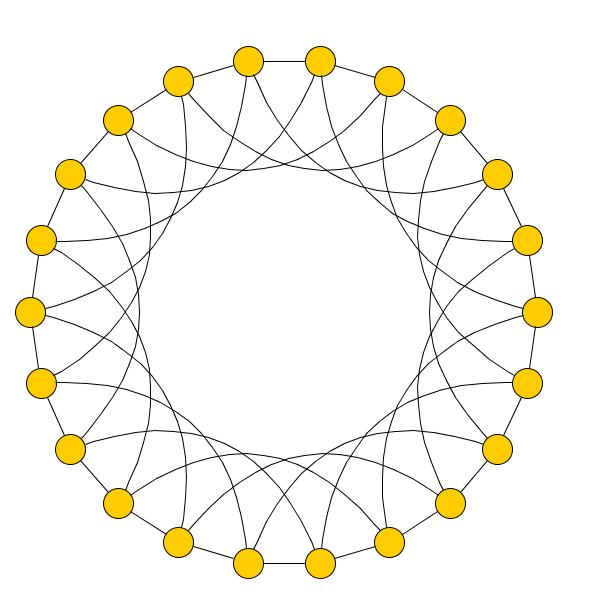
\includegraphics[width=0.4\textwidth]{figures/dloop.jpg}}
  \caption{A double Loop chordal ring C(1,4).}
\end{figure}
\item A {\em Triple Loop}   is a chordal ring  $C_n(1,p, k)$, with    $p<k$  and $k<\lfloor\frac{n}{2}\rfloor$. In other words, it is an augmented ring where each node has two additional chords at a distance of $\pm p$ and $\pm k$.
Therefore, each node has six neighbours: three in the counter-clockwise direction and three in the clockwise direction. 
\begin{figure}[H]
  \centering
    \reflectbox{%
      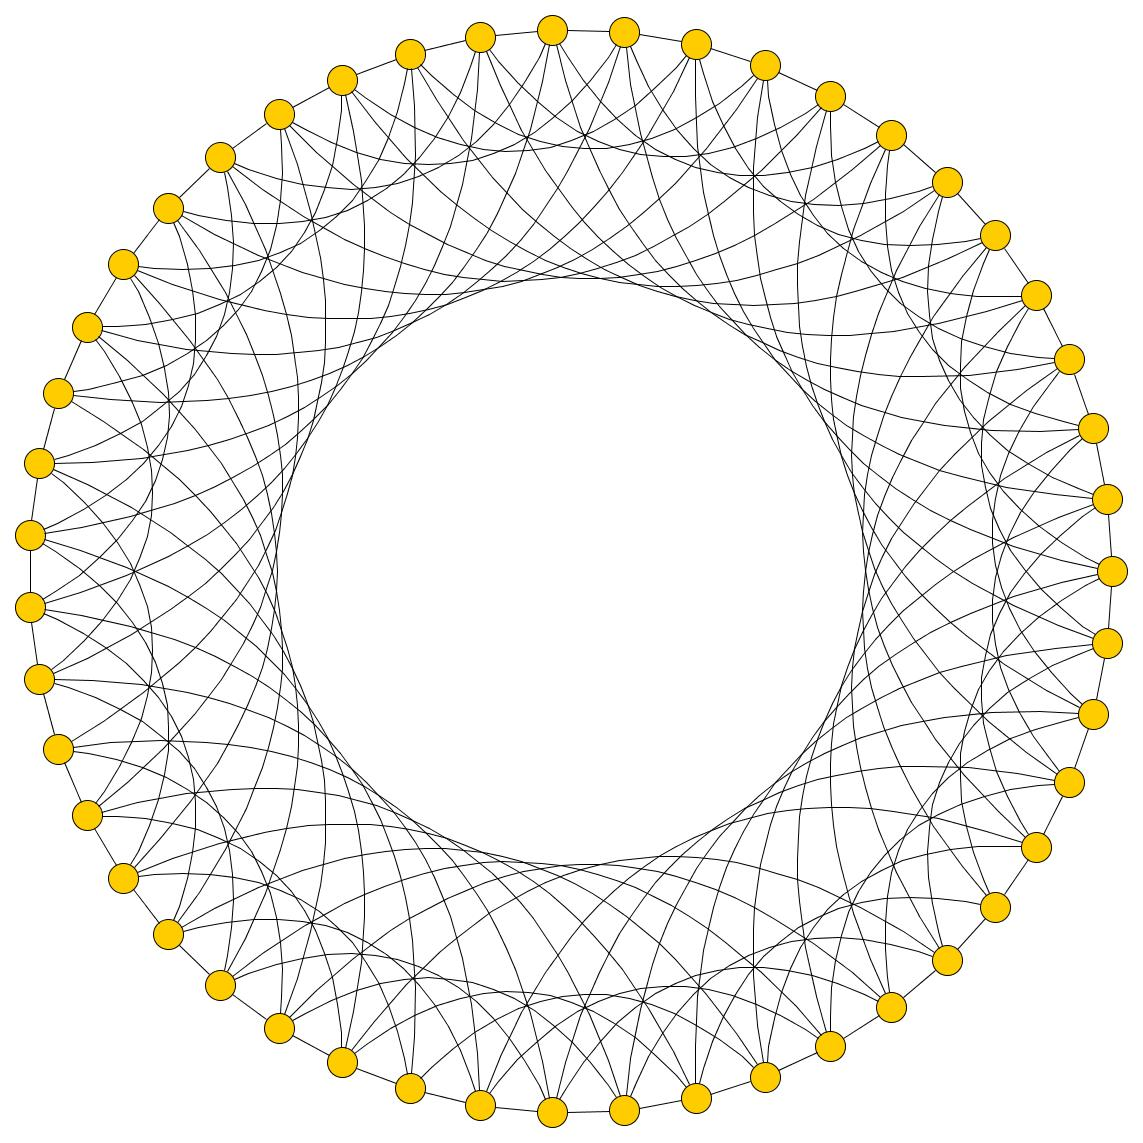
\includegraphics[width=0.4\textwidth]{figures/tloop.jpg}}
  \caption{A triple Loop chordal ring C(1,5,9).}
\end{figure}

\item A {\em Consecutive-Chords} is a chordal ring  $C_n(1,2,\ldots,k-1,k)$, with  $k < \lfloor\frac{n}{2}\rfloor$.
 In a  chorded ring, each node  has $2k$ consecutive  neighbours: $k$ neighbours in each direction. 
\begin{figure}[H]
  \centering
    \reflectbox{%
      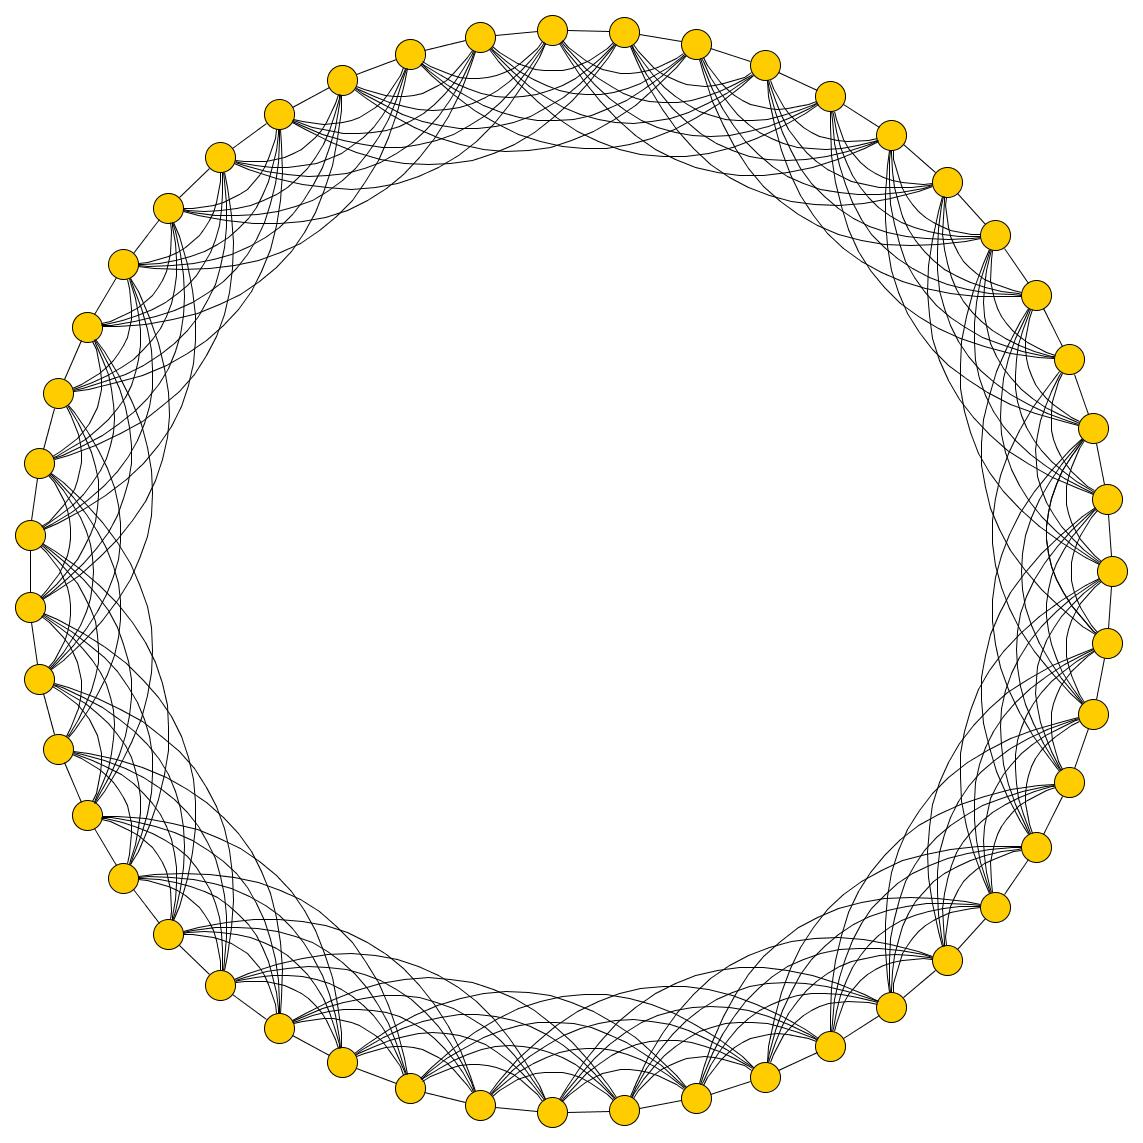
\includegraphics[width=0.4\textwidth]{figures/cloop.jpg}}
  \caption{A consecutive-chords chordal ring C(1,2,3,4,5).}
\end{figure}

\end{itemize}











\section{General Strategy}

 We now describe a general high level strategy that can be employed to solve  
  the \bv decontamination problem. 
  Our algorithm  can be divided into two phases: {\it Exploring and Shadowing} and {\it Surrounding and Eliminating}.

\subsection{Phase 1: Exploring and Shadowing}
The main goal of this phase is to determine the location of the original {\it black virus}. Since the location of the \bv is unknown a priori, we need to explore the topology until it is found. Finding the node in which the \bv resides implies triggering that {\it black virus}, creating new ones, destroying an agent in the process, and cleaning the node that contained the original  {\it black virus}. This process is done by the  leading exploration agent $LEA$, the exploring agent $EA$ and a group of shadow agents $SH$. 

 Starting from the  \hb, the leader and the exploring agent explore    the
 chordal ring by moving throughout the outer  ring  only. The assumption here is that the leader and the exploring agent are moving in a clockwise direction using the {\em safe exploration} technique:  $LEA$ and $EA$ are at safe node $v_{j}$, $EA$ moves to the next node $v_{j+1}$ while $LEA$ waits at $v_{j}$; if $EA$ returns to its leader then $v_{j+1}$ is not a \bv and they both move to $v_{j+1}$. If, while moving in this fashion,  $LEA$ receives a \bv instead of $EA$, then the location of the original \bv is detected and $EA$ is destroyed. 


  If node $v_i$ represents the node under exploration, $N(v_i) $ represents the neighbours of $v_i$, and  $N_{ex}(v_i) $  and $N_{un}(v_i)$ denote the set of explored and unexplored neighbours of node $v_i$. 
  The role of the shadow agents is to protect the already explored nodes from potential reinfection. When a new node $v_i$ is under exploration, the shadow agents should occupy its explored neighbours $N_{ex}(v_i)$.
Once $EA$ arrives to the \bv location it is destroyed, $LEA$ receives a $BV$ instead of EA, that node is cleared, and the new \bvs are now located on  all the unprotected (unexplored) neighbours of the \bv.
The set of nodes between the \hb and the node being explored is called the {\em safe area} and denoted by $S_{area}$. For  our protocol to be monotone, we have to insure that the nodes in the safe area do  not get re-infected. To do so,  the {\em   shadow agents} are deployed to guard the explored counter-clockwise neighbours of the next node to be visited. The deployment of $SH$s begins when $LEA$ and $EA$ have explored at least $d_2$ nodes. In other words, if $C_n( d_1=1, d_{2}, ..., d_{k})$
and $\left\vert{S_{area}}\right\vert \ge d_2$, at least one $SH$ is deployed and the number of $SH$s increases to match the number of neighbours of the currently explored node in the safe area. 
There is a section of the {\em safe area}  called the {\it danger area}, denoted by $D_{area}$, where $v_{n-1}\ge D_{area}\ge v_{n-d_k}$. In this area, the possibility of reinfection of explored nodes is increased. Because of this, we need $SH$s to guard the counter-clockwise neighbours as well as some or all of the clockwise neighbours.

Since all operations are synchronized, shadow agents are created at once and stay inactive until their timer reaches zero. In other words, all $SH$s have timers that have been set to different values in order to synchronize them with the exploring team ($LEA$ and $EA$). 
%to guard the explored neighbours of the node which is currently being explored. 
When the \bv is found the  $SH$s are notified by the $LEA$. 
%When the exploring team begins exploring nodes in the $D_{area}$, which is after $3(n-d_k)$ time units, $SH$(s) start their role to keep the protocol monotone.
Figure \ref{fig:ph1} shows an example of the first phase in a double loop. The green nodes represent the safe area and the red nodes represent the danger area.
\begin{figure}[H] 
  \centering
   
  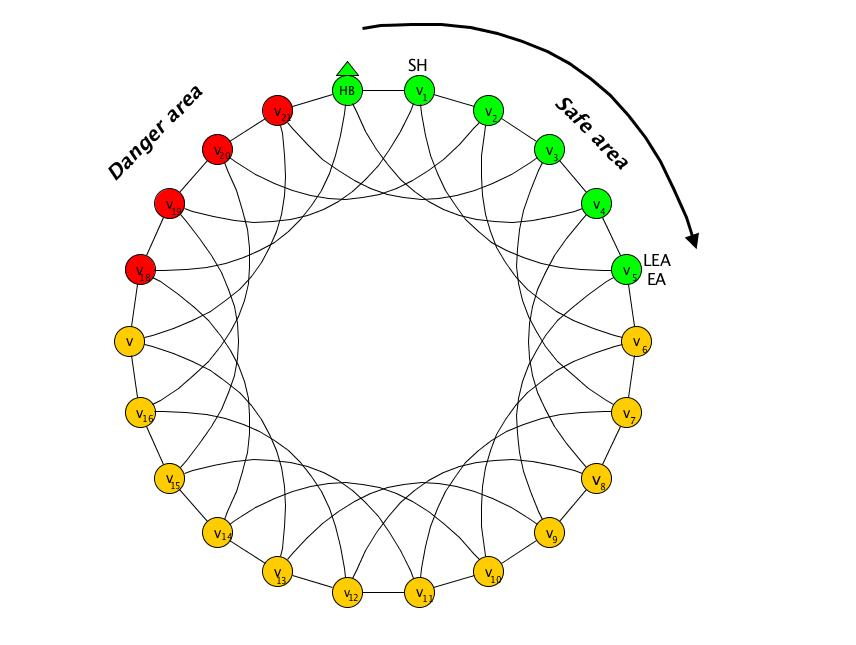
\includegraphics[width=0.6\textwidth]{figures/dloop_ph1.jpg}
  \caption{First phase in a double loop chordal ring C(1,4).} \label{fig:ph1}
\end{figure}






  \begin{center}
\fbox{
\begin{minipage}{6 cm}
{\sc  Exploring and Shadowing}
  \begin{tabbing}
let $HB= v_0$ \\
  Age\= nts $EA $ and $$LEA$$ at safe node  $v_i$.\\
 - Compute  $N_{ex}(v_{i+1})$ \\
 - For each $q \in N_{ex}(v_{i+1})$ \\
 \tab  $SH$ is deployed\\
 - $EA$ moves to $v_{i+1}$\\
 \tab If $EA$ returns back to $v_{i}$\\
 \tab \tab $LEA$ and $EA$ move to $v_{i+1}$\\
  \tab Else (i.e., $BV$ moves to $v_{i}$)\\
\tab \tab $EA$ is destroyed\\
 \tab \tab $BV=N_{un}(v_{i+1})$
  \end{tabbing}
\end{minipage}
}
\end{center}





This phase comes to an end when the \bv is detected and cleared; meanwhile, other \bvs have been created and moved to the unexplored neighbours of the original {\it black virus}. At this point, the second phase begins. The first phase is common to all of the strategies proposed in this thesis.



\subsection{Phase 2: Surrounding and Eliminating}
 
Once the \bv node is detected, $LEA$ moves to its location and the {\em Surrounding and Eliminating} phase begins. In this phase, the entire chordal ring is disinfected. The disinfection process is conducted by sending agents to the unexplored neighbours of the newly created {\it black viruses}. $LEA$ then sends $CA$(s) to activate those \bvs and  clear them. 

 First, let us introduce some notation. $x_0$ represents the original \bv. $V$ represents  the set of all vertices. The set of black viruses in the system is denoted by  ${\cal BV}$ .
${\cal S} = V - {\cal BV}$ represents the set of  nodes that does not contain any ${\cal BV}$. ${\cal T}$ represents the set of targets, that is, the nodes to be occupied. 

  \begin{center}
\fbox{
\begin{minipage}{7.5cm}
{\sc Surrounding and Eliminating} 
  \begin{tabbing}
 $$LEA$$ \= and  $SH$s  covering all $N_{ex}(v)$ \\
 $BV$ comes back from $v$. \\
  \> - Compute  $N_{un}(v)$\\
 \> - For \= each $u \in   N_{un}(v)$:\\
 \>\> Deploy  an  agent  to each  $z\in \{N(u)\setminus  N_{un}(v)\}$\\
 \>\> Wh\=en $N(u)$ is covered:\\
 \>\>\> Deploy one agent to   $u$
  \end{tabbing}
\end{minipage}
}
\end{center}



 In this phase, we need the same number of $SA$s as the number of neighbouring nodes of the {\it black viruses}. The $SA$s move to their destinations, and once all of the agents are in position, $LEA$ sends $CA$s to trigger all the \bvs at once. 


\begin{figure}[H]
  \centering  
  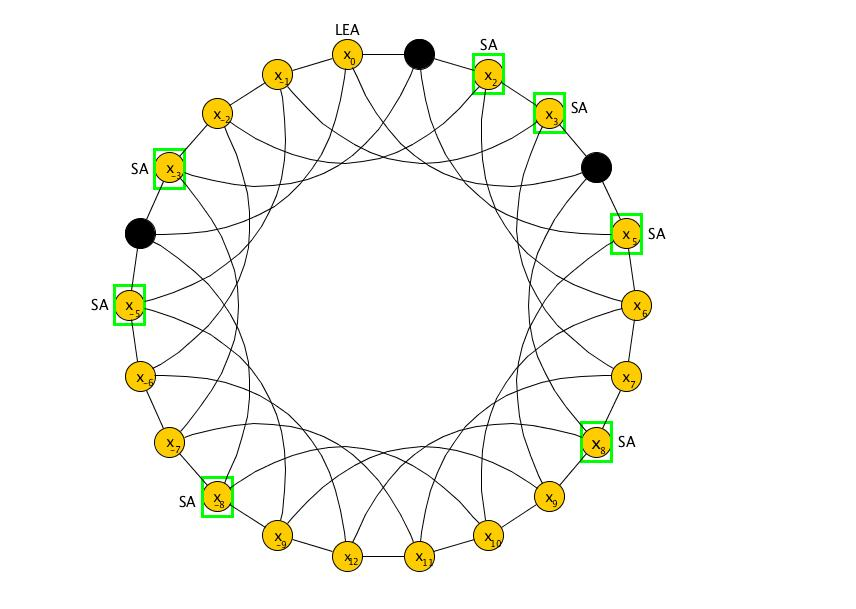
\includegraphics[width=0.6\textwidth]{figures/dloop_ph2.jpg}
  \caption{Location of SAs in  $C(1,4)$ where the black nodes represent the triggered black viruses.}\label{fig:second phase}
\end{figure}

Figure \ref{fig:second phase} shows the location of $SA$s  in a double loop after triggering the original {\it black virus} which then creates three more {\it black viruses} in the worst case.


Deploying agents is the most important part of this phase. Deployment can be done in different settings. In this thesis, we discuss two deployment strategy variations: {\em local} and {\em non-local}.

The non-local strategy that we propose  is called {\em Move-Optimal Deployment}. In this strategy, we assume that $LEA$ is the manager of the entire process. $LEA$ resides in node $x_0$, the location of the original {\it black virus}, where it sends the surrounding agents to their destinations through the shortest path.
Therefore, a surrounding agent carries the whole path starting from $x_0$ to any $t \in \cal T$. It is possible to devise a variant of this optimal strategy in which all agents have full topology information. In this case, there is no need for a surrounding agent to carry the full path while moving toward its target since the agent can re-compute it at each intermediate node. 
 
The local strategies are based on the {\em Greedy} approach.  Some of the greedy strategies are only applicable to certain  chord structures  because  they would not produce the correct routing when used with other structures. These strategies do not require as much storage as the non-local strategy since the surrounding agents do not carry paths to their destinations. Instead, they calculate their next step each time on the basis of their current location and the location of the target destination with no additional information. The local strategies that will be discussed in this thesis are: the {\it Simple Greedy}, the {\em Smart Greedy} and the {\em One-direction Greedy}.
In the {\it Simple Greedy} strategy, at each node the agent must decide the next node according to its distance from the target. In the {\em Smart Greedy} strategy,  the agents use more information in order to obtain better results. In the {\em One-direction Greedy} strategy, the agents move greedily in one direction until they reach their target. We will discuss each strategy in depth throughout this thesis. 



 \section{Conclusions}
 In this chapter we introduced our problem and some important definitions and terminologies. We also described the team of agents and their specific roles: coordinating, exploring, shadowing, surrounding and activating. Moreover, we  discussed the main topology of this thesis which is the chordal ring. Finally, we presented a general overview of the two phase solution: {\it Exploring and Shadowing} and  {\it Surrounding and Eliminating}. 

 
